\documentclass{article}
\usepackage[margin=1in]{geometry}
\usepackage{amsmath,amsthm,amssymb}
\usepackage{bbm,enumerate,mathtools}
\usepackage{tikz,pgfplots}
\usepackage{chessboard}
\usepackage[hidelinks]{hyperref}
\usepackage{multicol} % Problem 35

\newenvironment{question}{\begin{trivlist}\item[\textbf{Question.}]}{\end{trivlist}}
\newenvironment{note}{\begin{trivlist}\item[\textbf{Note.}]}{\end{trivlist}}
\newenvironment{references}{\begin{trivlist}\item[\textbf{References.}]}{\end{trivlist}}
\newenvironment{related}{\begin{trivlist}\item[\textbf{Related.}]\end{trivlist}\begin{enumerate}}{\end{enumerate}}


\begin{document}
\rating{3}{2}
  Consider walks on an $n \times m$ grid, where the walk can only self-intersect
  at a perpendicular step.
\begin{figure}[ht!]
  \centering
  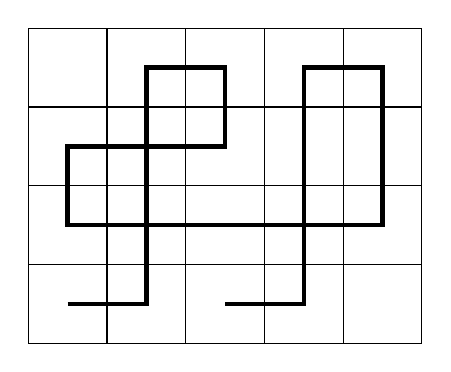
\begin{tikzpicture}
    \draw (0,0) grid (5,4);
    \draw[ultra thick] (0.5,0.5)--(1.5,0.5)--(1.5,3.5)--(2.5,3.5)--(2.5,2.5)--(0.5,2.5)--(0.5,1.5)--(4.5,1.5)--(4.5,3.5)--(3.5,3.5)--(3.5,0.5)--(2.5,0.5);
  \end{tikzpicture}
  \caption{An example of a walk on a $5 \times 5$ grid.}
\end{figure}

\begin{figure}[ht!]
  \centering
  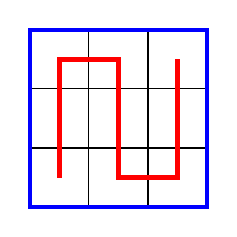
\begin{tikzpicture}[scale = 0.75]
    \draw (0,0) grid (3,3);
    \draw[ultra thick, blue] (0,0) rectangle (3,3);
    \draw[ultra thick, red] (0.5,0.5)--(0.5,2.5)--(1.5,2.5)--(1.5,0.5)--(2.5,0.5)--(2.5,2.5);
  \end{tikzpicture}
  ~
  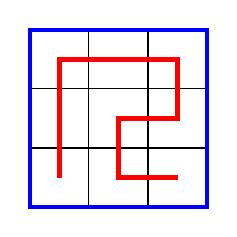
\begin{tikzpicture}[scale = 0.75]
    \draw (0,0) grid (3,3);
    \draw[ultra thick, blue] (0,0) rectangle (3,3);
    \draw[ultra thick, red] (0.5,0.5)--(0.5,2.5)--(2.5,2.5)--(2.5,1.5)--(1.5,1.5)--(1.5,0.5)--(2.5,0.5);
  \end{tikzpicture}
  ~
  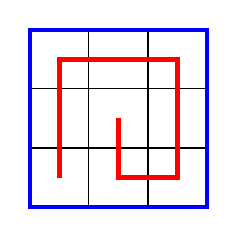
\begin{tikzpicture}[scale = 0.75]
    \draw (0,0) grid (3,3);
    \draw[ultra thick, blue] (0,0) rectangle (3,3);
    \draw[ultra thick, red] (0.5,0.5)--(0.5,2.5)--(2.5,2.5)--(2.5,0.5)--(1.5,0.5)--(1.5,1.5);
  \end{tikzpicture}
  ~
  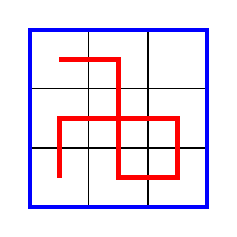
\begin{tikzpicture}[scale = 0.75]
    \draw (0,0) grid (3,3);
    \draw[ultra thick, blue] (0,0) rectangle (3,3);
    \draw[ultra thick, red] (0.5,0.5)--(0.5,1.5)--(2.5,1.5)--(2.5,0.5)--(1.5,0.5)--(1.5,2.5)--(0.5,2.5);
  \end{tikzpicture}
  ~
  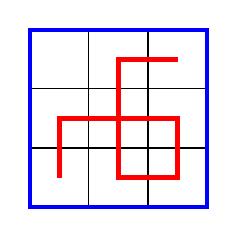
\begin{tikzpicture}[scale = 0.75]
    \draw (0,0) grid (3,3);
    \draw[ultra thick, blue] (0,0) rectangle (3,3);
    \draw[ultra thick, red] (0.5,0.5)--(0.5,1.5)--(2.5,1.5)--(2.5,0.5)--(1.5,0.5)--(1.5,2.5)--(2.5,2.5);
  \end{tikzpicture}
  ~
  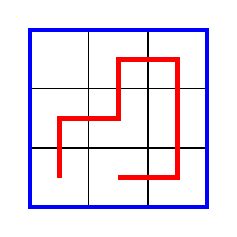
\begin{tikzpicture}[scale = 0.75]
    \draw (0,0) grid (3,3);
    \draw[ultra thick, blue] (0,0) rectangle (3,3);
    \draw[ultra thick, red] (0.5,0.5)--(0.5,1.5)--(1.5,1.5)--(1.5,2.5)--(2.5,2.5)--(2.5,0.5)--(1.5,0.5);
  \end{tikzpicture}
  \caption{
    Six (all?) ``as-long-as-possible'' paths starting in the lower left corner,
    up to dihedral action on the $3 \times 3$ grid.
  }
\end{figure}

\begin{question}
  How many $n \times n$ boards exist with a unique solution?
\end{question}

\begin{related}
  \item What if paths must be ``as long as possible'', in the sense that they
    can't be extended at either end? Exactly $k$ steps?
  \item What if this is done on a torus, triangular grid, cube, etc?
  \item What if paths much touch every square at least once?
  \item How many up to dihedral action? How many with dihedral symmetry?
  \item What if paths must start at, say, the upper right corner?
  \item What if the path must have at least one self-intersection?
  \item What if paths are allowed to be loops (i.e., end on same square as they
    began on?) What if they must be loops?
  \item What is the greatest number of king steps?
    Fewest on an ``as-long-as-possible'' path? Rook steps?
  \item What if diagonal moves are allowed? Only diagonal moves?
  \item What if multiple paths can be drawn on the same grid, only intersecting perpendicularly?
\end{related}

\begin{references}
  \item Special case of Problem 31. Problem 42 and 56.
  \item Pipe Mania puzzle game. \url{https://en.wikipedia.org/wiki/Pipe_Mania}
\end{references}

\end{document}
